\documentclass[12pt]{beamer}
\usepackage[utf8]{inputenc}
\usepackage[T1]{fontenc}
\usepackage{lmodern}
\usepackage[spanish]{babel}
\usepackage{amsmath}
\usepackage{amsfonts}
\usepackage{amssymb}
\usepackage{graphicx}
\usepackage{hyperref}
\usepackage{multicol}
\usepackage{dirtree}
\usepackage{listings}
\usepackage{etoolbox} % to reduce spacing in bearmers toc
\usetheme[block=fill]{metropolis}

\begin{document}
	\author{Fernando Oleo Blanco \\ fernando.oleo@alu.comillas.edu \hfill 	\href{https://github.com/Irvise/Documents}{github.com/Irvise/Documents}}
	\title{Introducción a \textrm{\LaTeX}}
	%\subtitle{}
	%\logo{}
	\institute{(ICAI - LinuxEC) DEP}
	\date{\today}
	%\subject{}
	%\setbeamercovered{transparent}
	\setbeamertemplate{navigation symbols}{}
	\setbeamertemplate{footline}[page number]
\begin{frame}[plain]
	\maketitle
\end{frame}

\begin{frame}{Índice}
%\vfill
\tableofcontents
%\clearpage
\end{frame}

\begin{frame}{Resumen}
\begin{enumerate}
	\item Diseño del documento
	\item Configuración del documento
	\item Estructuración del texto
	\item Herramientas para el trabajo de texto
	\item Entornos útiles
	\item Referencias y bibliografía
	\item Escritura científica
	\item Recursos extra
\end{enumerate}
\end{frame}

\section{Historia}

\begin{frame}[plain]
	\begin{figure}
		\centering
		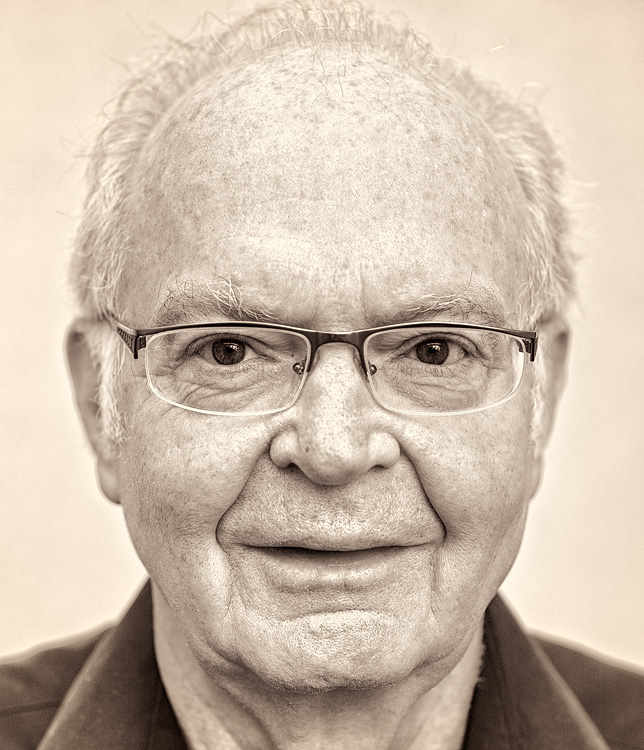
\includegraphics[height=0.75\linewidth]{Donald-Knuth-Stanford-Computer-Science}
		\caption{Donald Ervin Knuth. Creador de \TeX}
		\label{fig:donald}
	\end{figure}
\end{frame}

\begin{frame}{Un pequeño cuento}
\small
\begin{block}{¿Quién es Knuth?}
	Americano. Profesor de Stanford, ya retirado. Matemático, físico, informático y teólogo. Actualmente escribe la serie de libros \texttt{The Art of Computer Programming,} precursora del nacimiento de \TeX. Considerado uno de los padres de la informática moderna
\end{block}

\begin{block}{\TeX}
	Después de crear el segundo volumen y empezar el tercero se dio cuenta que la tipografía carecía calidad. Buscó soluciones y decidió estudiar tipografía para crearse su propio sistema. \TeX es el entorno de programación, \LaTeX\ es \TeX\ y unos paquetes para agilizar su escritura
\end{block}

	\textit{"Si una herramienta que uso la utilizan muchas personas, seguramente pensaría que estoy haciendo algo mal"}

\end{frame}

\section{Instalación y recursos}

\begin{frame}{Instalación}

\begin{block}{TexStudio, IDE}
	$\bullet$ \href{http://www.texstudio.org/}{\textbf{\TeX Studio:}} Download $\rightarrow$ busca tu plataforma. Instálalo como solo tú sabes
\end{block}

\begin{block}{\LaTeXe}
	$\bullet$ \href{https://www.latex-project.org/get/}{\textbf{"Compilador"}} \\
	Windows: usad o Mik\TeX\ o Texlive. Texlive es el tradicional\\
	Mac: instalad Mac\TeX\ y listo
	Linux: buscad \texttt{texlive} en buestra distribución
\end{block}
\begin{block}{Recursos on-line}
	Accesibles desde el link anterior. Es una buena idea tener una copia en la nube. Recomiendo \href{https://www.overleaf.com/}{Overleaf,} recientemente fusionado con Share\LaTeX
\end{block}
\end{frame}

\begin{frame}{Recursos recomendados}
\begin{block}{Lectura}
	$\bullet$ \href{https://tobi.oetiker.ch/lshort/lshort.pdf}{\textit{The not so Short Introduction to \LaTeX}} por Tobias Oetiker \\
	$\bullet$ \href{https://en.wikibooks.org/wiki/LaTeX}{\textit{\LaTeX\ Wikibook:}} Libro escrito por y para Wikipedia. El 99\% de vuestras dudas tienen solución aquí \\
	$\bullet$ \href{http://osl.ugr.es/CTAN/info/Math_into_LaTeX-4/Short_Course.pdf}{\textit{More Math Into \LaTeX}} por George Grätzner (esta es una buena muestra)
\end{block}
\begin{block}{Internet}
	$\bullet$ Cualquier servicio con plantillas (\href{http://www.latextemplates.com/}{\textbf{Latextemplates}} por ejemplo) \\
	$\bullet$ \href{https://www.tug.org/begin.html}{\textbf{Tug:}} Centro de recursos \textit{oficiales} \\
	$\bullet$ Foros (\href{https://www.overleaf.com/learn}{\underline{\textbf{Overleaf-learn}}}), "puntos de información", etc \\
	$\bullet$ Google
\end{block}

\end{frame}

\section{Comparativa con Word}

\begin{frame}[t]{Diferencias notables}
	\begin{columns}[t]
		\begin{column}{0.4\textwidth}
			Microsoft Word
			\begin{itemize}
				\item Intuitivo, fácil de usar
				\item Ya conocido
				\item Imágines, tablas, etc se hacen solas \\
				\hrulefill
				\item ¿Bibliografía?
				\item ¿Índice?
				\item ¿Referencias?
			\end{itemize}
		\end{column}
		\begin{column}{0.55\textwidth}
			\LaTeX
			\begin{itemize}
				\item Complicado, tedioso
				\item Con un error, ya nada funciona
				\item Escribirlo todo manualmente...\\
				\hrulefill
				\item Estructura automática
				\item Texto de calidad sin esfuerzo
				\item No da problemas las dos semanas antes de la entrega
			\end{itemize}
		\end{column}
	\end{columns}
\end{frame}

\begin{frame}{Buenas prácticas generales}
	\large
	\begin{enumerate}
		\item Cuando algo falla, \textbf{leed el mensaje de error}
		\item Nunca, nunca, nunca empecéis desde cero. \textbf{¡Usad plantillas!}
		\item Sed organizados
		\item \textbf{Haced las cosas sencillas}, si no es obvio, no lo hagas
		\item Buscad ayuda (en mi o en los recursos mencionados)
		\item ¡Comentad lo que hacéis! \% Comentario
		\item \textbf{Leed la documentación}
		\item \textbf{Usad bien el IDE.} ¡Ahorra un montón de tiempo! 
	\end{enumerate}
\end{frame}

\section{Estructura del documento}

\begin{frame}{Estructura de archivos para el trabajo}
	Estructura de archivos recomendada. Es la que usa la plantilla
	\begin{columns}
		\begin{column}{0.4\textwidth}
			\dirtree{%
				.1 /. 
				.2 main.tex. 
				.2 biblio.bib. 
				.2 \dots. 
				.2 Cap1. 
				.3 cap1.tex. 
				.3 img.png. 
				.3 main.pdf. 
				.3 \dots. 
				.2 Cap2. 
				.3 \dots. 
			}
		\end{column}
		\begin{column}{0.6\textwidth}
			En \LaTeX\ podemos, y se recomienda, dividir nuestro archivo en partes pequeñas y en carpetas. Esto permite estructurar mucho mejor el documento, mantener los archivos ordenados, y trabajar con textos menores.
		\end{column}
	\end{columns}
\end{frame}

\subsection{\texttt{\ documentclass y preámbulo}}

\begin{frame}[fragile, allowframebreaks]{Estructura general de los comandos}
	\begin{block}{Comando simple}
		Comienzan con $\textbackslash$, seguido del comando. Si este comando recibe algún argumento (o algunos), estos van entre llaves. Si reciben opciones, van entre corchetes antes del argumento. Ejemplos: \\
		\verb|\hrulefill| $\rightarrow$ \hrulefill \\
		\verb|\textit{Hola}| $\rightarrow$ \textit{Hola} \\
		\verb|\textcolor{blue}{azul}| $\rightarrow$ \textcolor{blue}{azul}
	\end{block} \pause
	\begin{block}{Entornos}
		Como comandos normales, pero cuya función es más extensa y compleja; tienen la estructura: \verb|\begin{entorno}[opciones]{argumento}| \\ \verb| content... | \\ 
	\verb|\end{entorno}|. En IDE \texttt{Crtl + e}
	\end{block}
\end{frame}

\begin{frame}[fragile]{Comienzo de nuestro documento}
	\begin{block}{\textbf{\texttt{$\textbackslash$documentclass}}}
		\underline{\textbf{Nuestra primera línea.}} Define la naturaleza de nuestro documento. Ejemplo:  \verb|\documentclass[12pt, a4paper, ...]{book}|
	\end{block}
	\begin{columns}
		\begin{column}{0.5\textwidth}
			\textbf{Argumentos}
			\begin{itemize}
				\item \texttt{article}
				\item \texttt{book}
				\item \texttt{letter}
				\item \texttt{beamer}
				\item $\vdots$
			\end{itemize}
		\end{column}
		\begin{column}{0.5\textwidth}
			\textbf{Opciones}
			\begin{itemize}
				\item Tamaño letra: \texttt{10pt}
				\item Orientación: \texttt{landscape}
				\item Columnas: \texttt{twocolumn}
				\item Centrado: \texttt{twoside}
				\item $\vdots$ \texttt{draft, openright...}
			\end{itemize}
		\end{column}
	\end{columns}
\end{frame}

\begin{frame}[fragile]{Importación de herramientas, $\textbackslash$\texttt{usepackage\{\}}}
	En \LaTeX\ se expande la funcionalidad mediante paquetes, algunos son \textbf{\underline{muy}} necesarios. Esta sección debería ir justo debajo del \texttt{documentclass}
	\verb|\usepackage{geometry} % Ajusta geometrías| \\
	\verb|\usepackage[spanish]{babel} % Formato en castellaño|
	\verb|"{graphicx} % Imágenes, pdfs, etc|
	\verb|"{hyperref} % Referencias como tienen que ser|
	\verb|"[utf8]{inputenc} % Tíldes y otros caracteres|
	\verb|"{amsmath, amssymb} % Escritura científica| \\
	\hrulefill\\
	\textbf{Ver también:} \texttt{makeidx (índices avanzados), fancyhdr (cabeceras y pie de página), multicol (columnas personalizadas), booktabs (para tablas preciosas)}
\end{frame}

\begin{frame}[fragile]{Datos previos al documento escrito, preámbulo}
Como \LaTeX\ hará un buen número de cosas automatizadas, le damos unos datos generales en el preámbulo para que el los trate como deba.
\begin{block}{Información del autor y texto}
	\verb|\author{Fernando ... \and Miguel \thanks{...}}| \\
	\verb|\title{Título}| \\
	\verb|\date{\today} % O en blanco si no se quiere|
\end{block}
\begin{block}{Secuencias de diseño o configuración}
	Si estuviéramos usando \texttt{fancyhrd, makeidx o similares} tendríamos que escribir en el preámbulo su diseño o configuración.
\end{block}
\end{frame}

\begin{frame}{En resumen}
	\textbf{Comienzo:} \texttt{documentclass}
	\vfill
	\textbf{Paquetes:} \texttt{usepackage}
	\vfill
	\textbf{Preámbulo:} \texttt{configuraciones generales}
\end{frame}

\subsection{Manejo del texto}

%\begin{frame}[fragile]{Comienzo del texto}
%	\textbf{TODO} el documento se encontrará entre \begin{verbatim}
%	\begin{document}
%	\end{document}
%	\end{verbatim}
%	Comenzamos con:
%	\begin{verbatim}
%		\begin{document}
%		\begin{titlepage} % Portada
%		\maketitle % Generación de portada automática
%		\thispagestyle{empty} % Para que no salga numerada
%		\begin{abstract}
%		Resumen inicial (abstract). Formateo automático
%		\end{abstract}
%		\end{titlepage}
%	\end{verbatim}
%\end{frame}
%
%\begin{frame}[fragile]{Cont.}
%	\begin{verbatim}
%		Cont.
%		\cleardoublepage % Nueva página e inicio en derecha
%		\pagenumbering{Roman} % Numeración romana
%		\tableofcontents % Esta estructura es un ejemplo
%		\newpage
%		\listoffigures % Estos tres comandos también se 
%		\newpage
%		\listoftables % suelen poner en el apéndice
%		\newpage
%		\listoflistings % Para código
%		\pagenumbering{arabic} % Numeración arábica
%	\end{verbatim}
%\end{frame}
%
%\begin{frame}[fragile]{Cont.}
%	Recordemos que en \LaTeX\ se puede dividir el texto. Las partes se incluyen con: \verb|\include{file}|
%	\begin{verbatim}
%		Cont.
%		% Ahora podemos importar los distintos archivos
%		\include{Cap1/cap1} % Incluimos el archivo de la
%		% carpeta Cap1. El archivo va sin extensión .tex
%		\include{Cap2/cap2} 
%		% Etcétera
%		\appendix % Iniciamos apéndice
%		\include{lo_que_sea}
%		% Incluir bibliografía (se verá después el cómo)
%	\end{verbatim}
%\end{frame}

\begin{frame}[fragile]{Seccionamiento del texto}
	\begin{block}{En la clase \texttt{book}, se tienen principalmente tres niveles}
		\verb|\chapter[short title]{title}| \\
		\verb|\section[short title]{text}|\\
		\verb|\subsection[short title]{text}|\\
		-\verb|\subsubsection[short title]{title}|-
	\end{block}
	
	\texttt{[short title]} es lo que aparecería en el índice y en el encabezado. \\ 
	
	Si no se quiere numerado ni en el índice: \verb|\section*{title}|\\
	\hrulefill\\
	Para escribir párrafos, dejar una línea en blanco entre ellos. Para romper una línea usar \verb|\\|
\end{frame}

\begin{frame}[fragile]{Estilos de texto}
	\texttt{C:} control, \texttt{S:} shift
	\begin{block}{Los más comunes y recomendados}
		\begin{description}
			\item[Negrita/Boldface] \verb|\textbf{text}| \textbf{text}. En IDE \texttt{C + b}
			\item[Cursiva/Énfasis] \verb|\emph{text}| \emph{text}. En IDE \texttt{C + S + e}
			\item[Subrayado] \verb|\underline{text}| \underline{text}.
			\item[SmallCaps] \verb|\textsc{text}| \textsc{text}. En IDE \texttt{C + S + c}
			\item[Typewritter] \verb|\texttt{text}| \texttt{text}. En IDE \texttt{C + S + t}
		\end{description}
	\end{block}
\end{frame}

\begin{frame}[fragile, allowframebreaks]{Otras herramientas útilies}
	\begin{block}{Medidas y espaciados. No los deberíais necesitar}
		\begin{itemize}
			\item \verb|\hfill| rellena espacio horizontal.
			\item \verb|\vfill| ídem, pero en vertical.
			\item \verb|\hspace{text}| espaciado horizontal (usar \texttt{em como medida}). Tienen versiones forzadas.
			\item \verb|\vspace{text}| ídem pero en vertical. Ambos permiten valores negativos.
			\item \verb|\hrulefill|
		\end{itemize}
		\hrulefill
	\end{block}
	\begin{block}{Cont. medidas ``programáticas"}
		\begin{itemize}
			\item \verb|\textwidth| ancho del texto disponible (permite operaciones matemáticas). \verb|\columnwidth| es el ancho de la columna.
			\item \verb|\textheight| altura de la zona de texto.
			\item \verb|\linewidth| como \verb|\textwidth| pero relativo al entorno de trabajo
		\end{itemize}
	Estas son muy útiles para su uso con figuras o en tablas
	\end{block}
	\begin{block}{Bloques \textit{(boxes)}}
		Hay una buena ristra. El más importante, que puede que necesitéis, es \verb|\mbox{text}|. Este forma un bloque único inseparable (útil para, por ejemplo, nombres propios o números).
	\end{block}
	\begin{block}{Notas a pie de página}
		\verb|\footnote{text}|. Las notas a pie de página van integradas en el texto y su formato es automático. Por ejemplo\footnote{Damos una aclaración}. \\ \hrulefill \\
		\verb|Por ejemplo\footnote{Damos una aclaración}.|
	\end{block}
\end{frame}

\subsubsection{Entornos comunes}

\begin{frame}[fragile, allowframebreaks]{Tablas}
		\begin{block}{Entorno tabular/array básico}
		Esto es una introducción básica, pero suficiente, cubrirá vuestras necesidades. El IDE tiene una herramienta para hacer tablas \textit{ala} Excel.
		\verb|\begin{tabular}[opciones]{alineacion}|\\
		\texttt{contenido}\\
		\verb|\end{tabular}|\\
		
		\texttt{p, m, b} sirven para hacer párrafos (top, middle, bottom)
	\end{block}
	Ejemplo: 
	\begin{tabular}{l||c|r}
		11            &  12   &            13 \\
		\hline\hline
		hola          & hola  &          hola \\
		\hline
		adiós querida & adiós & Sayonara Baby
	\end{tabular}
	\begin{block}{Código anterior (el espaciado lo da el editor)}
		\vspace*{-1em}\begin{verbatim}
		\begin{tabular}{l||c|r}
		11            &  12   &            13 \\
		\hline \hline
		hola          & hola  &          hola \\
		\hline
		adiós querida & adiós & Sayonara Baby
		\end{tabular}
		\end{verbatim}\vspace*{-1em}
	\end{block}
	El \texttt{\&} es bien importante, es el símbolo de separación y alineación. \\
	\textbf{Nota:} ver \href{https://www.ctan.org/pkg/booktabs/}{\texttt{booktabs}}, \href{https://tex.stackexchange.com/questions/163061/help-with-a-booktabs-table}{(ejemplo)}
\end{frame}

\begin{frame}[fragile, allowframebreaks]{Items, enumeraciones y descripciones/listas}

\begin{block}{Items}
	\begin{columns}
		\begin{column}{0.5\textwidth}
			\begin{itemize}
				\item Para \verb|\item| automático en IDE \texttt{C + S + i}
				\item[Newww] Ejemplo bastante largo para que se vean las diferencias
				\item Otro item
			\end{itemize}
		\end{column}
		\begin{column}{0.35\linewidth}
			\begin{verbatim}
				\begin{itemize}
				\item Para ...
				\item[Newww] E...
				\item Otro item
				\end{itemize}
			\end{verbatim}
		\end{column}
	\end{columns}
\end{block}

\begin{block}{Enumeraciones}
	\begin{columns}
		\begin{column}{0.35\textwidth}
			\begin{enumerate}
				\item Ejemplo
				\item Cont.
				\begin{enumerate}
					\item Anidados
				\end{enumerate}
			\end{enumerate}
		\end{column}
		\begin{column}{0.4\linewidth}
			\begin{verbatim}
			\begin{enumerate}
			\item Para ...
			\item Cont.
			\begin{enumerate}
			\item Anidados
			\end{enumerate}
			\end{enumerate}
			\end{verbatim}
		\end{column}
	\end{columns}
\end{block}

\begin{block}{Descripciones/listas}
	\begin{columns}
		\begin{column}{0.4\textwidth}
			\begin{description}
				\item[label muy largo] Ejemplo de texto un tanto largo para que se vean las diferencias
				\item[Nombre muy largo] Descripción del texto
			\end{description}
		\end{column}
		\begin{column}{0.4\linewidth}
			\begin{verbatim}
			\begin{description}
			\item[label] Ejem...
			\item[Nombre] Cont.
			\end{description}
			\end{verbatim}
		\end{column}
	\end{columns}
\end{block}
\end{frame}

\begin{frame}[fragile]{Imágenes u otros elementos gráficos (pdfs)}
	\begin{block}{La imagen al inicio de la presentación}
		\vspace*{-1em}
		\begin{verbatim}
		\begin{figure}[h] % Opciones h, t, b, c
		\centering
		\includegraphics[height=0.75\linewidth]{Donald...}
		\caption{Donald Ervin Knuth. Creador de \TeX}
		\label{fig:donald-knuth-stanford-computer-science}
		\end{figure}
		\end{verbatim}\vspace*{-1em}
	\end{block}
	\texttt{includegraphics} nos da opciones para el control de la altura, ancho y escala. Sirve para un buen número de formatos, incluido \texttt{.pdf}. \verb|\caption[short title]{text}| es el texto que aparece debajo de la imagen y en la \texttt{tof.} \textbf{Usad el \textit{wizard} que trae el IDE.}
\end{frame}

\begin{frame}[fragile]{Programas y fragmentos de código}
	Se usa \verb|\usepackage{listings}|. Es personalizable hasta el final, desde color del fondo, esquemas de color para el código, reconoce docenas de lenguajes, etc. \textbf{Por favor,} miraros la documentación y copiad ejemplos.
	\begin{columns}
		\small
		\begin{column}{-\textwidth}
			\begin{lstlisting}[language=Pascal]
			for i:=maxint to 0 do
			begin
			{ do nothing }
			end;
			Write('Case insensitive ');
			Write('Pascal keywords.');
			\end{lstlisting}
		\end{column}
		\hspace*{-3em}\begin{column}{\textwidth}
			\begin{verbatim}
			\begin{lstlisting}[language=Pascal]
			for i:=maxint to 0 do
			begin
			{ do nothing }
			end;
			Write('Case insensitive ');
			Write('Pascal keywords.');
			\end{lstlisting}
			\end{verbatim}
		\end{column}
	\end{columns}
\end{frame}

\subsection{Referencias y bibliografía}

\begin{frame}[fragile, allowframebreaks]{Referencias}
	\vspace*{-0.5em}
	\begin{block}{\texttt{Labels,} etiquetado}
		\verb|\label{key}| nos permite etiquetar lo que deseemos referenciar (anterior o posteriormente). Ejemplos:
		\begin{itemize} 
			\item \verb|\label{eq:maxwell}| ecuación de Maxwell
			\item \verb|\label{fig:imagen}| alguna imagen
			\item \verb|\label{tab:tabla}| alguna tabla
			\item \verb|\label{sec:appendixa}| apéndice A
			\item Etcétera
		\end{itemize}
		Usadla/Indicádla a continuación de lo que queráis citar, dentro del entorno.
	\end{block}

	\begin{block}{Referencias, citas}
		\verb|\autoref{key}| nos generará la referencia de manera automática. Tendrá en cuenta el entorno usado, sección, etc. Ver Figura \autoref{fig:donald}. \\
		\vspace{1em}
		La forma tradicional sería con \verb|\ref{text}|: \verb|\ref{fig:donald}|. Lo que daría solo "\ref{fig:donald}", por lo que tendríamos que indicar qué estamos referenciando.
	\end{block}
\end{frame}

\begin{frame}[fragile, allowframebreaks]{Bibliografía, programas externos}
	\small
	No son necesarios para trabajar en \LaTeX\ como veremos. Pero son muy útiles para el manejo de bibliografías grandes y complicadas. Además de traer muchas herramientas de búsqueda y formato de gran ayuda. \\
	\hrulefill \\
	Recordad que hay servicios bibliográficos, como \href{https://scholar.google.com/}{\textbf{Google Scholar,}} donde podemos buscar la información de las referencias. Además, todos estos servicios sacan formato \textrm{Bib\TeX.} \\
	\hrulefill \\
	Nota, hay varios procesadores internos de bibliografía, nosotros usaremos el más flexible y sencillo:  \textrm{Bib\LaTeX.} \\ \textbf{Comentar configuración en \TeX Studio}
	
	\begin{block}{Programas}
	\begin{description}
		\item[\href{https://www.zotero.org/}{Zotero}] Multiplataforma y exporta tanto a \LaTeX\ como a Word. Todas las herramientas necesarias están incluidas excepto un motor de búsqueda con texto (puede ISBNs, DOIs, etc), aunque tiene integración con Firefox y Safari.
		\item[\href{http://www.jabref.org/}{JavRef}] Multiplataforma y también exporta a Word. Completo y avanzado. También tiene integración con Firefox.
		\item[\href{https://userbase.kde.org/KBibTeX}{KBibTeX}] Solo Linux. Muy simple pero sencillo de usar y flexible, además de traer varios motores de búsqueda.
	\end{description}	
	\end{block}
	\vspace*{-3em}
\end{frame}

\begin{frame}[fragile, allowframebreaks]{Bibliografía en \LaTeX, uso en el documento}
	\begin{block}{Citas}
		Para citar una obra simplemente se hace \verb|\cite{bibid}| donde se quiera la referencia. El \texttt{bibid} es el identificador de nuestra referencia.
	\end{block}

	\begin{block}{Inclusión en el documento y estilos}
		\begin{verbatim}
		\section{Bibliografía}
		\bibliographystyle{style} % plain, abbrv, alpha...
		\bibliography{bib1,bib2,bib...} % Añadimos
		%  archivo(s), sin espacios ni extensión
		\end{document} % si queremos terminar
		\end{verbatim}
	\end{block}

	\begin{block}{Estructura del archivo \texttt{.bib}}
		Todas las entradas empiezan con una @ y su identificador (\texttt{article, journal, book, etc}); esto sirve para darles formato. A continuación se abren llaves. \\
		Entre las llaves se escribirá la información separada por comas. Lo \underline{más importante} es la primera palabra que pondremos, esa será la identificación para el comando \verb|\cite{bibid}|. A continuación rellenaremos tantos campos como necesitemos \texttt{año, título, autor, url, editor, etc}, tal y como está indicado en el ejemplo.
	\end{block}
	\vfill
	
	\small
	\begin{block}{El archivo \texttt{.bib}}
		El archivo \texttt{.bib,} que se recomienda que esté junto con el documento \texttt{.tex} principal, es nuestra \textit{base de datos} con las referencias. Un ejemplo sería:
		\vspace{-1.4em}
		\begin{verbatim}
		@BOOK{White201501,
		title={Fluid Mechanics},
		author={Frank M. White},
		publisher={McGraw-Hill Education},
		year={2015},
		edition={8},
		isbn={9780073398273},
		totalpages={864},
		timestamp={2018.10.29},
		}
		\end{verbatim}
		\vspace{-1.4em}
	\end{block}
	\vspace{-1.4em}
	\normalsize
\end{frame}

\section{Escritura científica}

\begin{frame}[fragile]{Lógica de la escritura científica en \LaTeX}

	\begin{block}{Desarrollo}
		$\bullet$ \LaTeX\ se creó para permitir una fácil y rápida creación de textos, aunque parezca poco intuitivo al principio. \\
		\textbf{Regla de la mano derecha:} si algo es muy utilizado y básico en el mundo de las matemáticas y de las ciencias, está acortado, simplificado. El resto son los nombres descriptivos. \textbf{Ejemplo:} la integral cerrada se usa mucho $\rightarrow$ está simplificada: $$\oint = \verb|$\oint$|$$ La doble integral cerrada sigue su desarrollo, pero no viene en Amsmath: \verb|$\oiint$|. La flecha a la derecha no es un símbolo matemático muy querido $\rightarrow$ no se abrevia \verb|$\rightarrow$|
	\end{block}
\end{frame}

\begin{frame}[fragile]{Ejemplos de lógica}
\vspace*{0.75em}
\begin{columns}
	\begin{column}{0.4\textwidth}
		\textbf{Expresivos}
	\begin{itemize}
			\item $\phi$ \verb|$\phi$|
			\item $\varphi$ \verb|$\varphi$|
			\item $\Phi$ \verb|$\Phi$|
			\item $\downarrow$ \verb|$\downarrow$|
			\item $\Downarrow$ \verb|$\Downarrow$|
		\end{itemize}
		\textbf{Abreviados}
		\begin{itemize}
			\item $\prod$ \verb|$\prod$|
			\item $\neq$ \verb|$\neq$|
			\item $\in$ \verb|$\in$|
			\item $\ni$ \verb|$\ni$|
		\end{itemize}
	\end{column}
	\begin{column}{0.6\textwidth}
		\textbf{Ejercicio, adivinad los símbolos}
		\begin{itemize}
			\item $\sim$
			\item $\Pi$
			\item $\pm$
			\item $\mp$
			\item $\rightarrow$
		\end{itemize}
		\pause
		\textbf{Respuestas}
		\begin{itemize}
			\item \verb|$\sim$|
			\item \verb|$\Pi$|
			\item \verb|$\pm$|
			\item \verb|$\mp$|
			\item \verb|$\rightarrow$|
		\end{itemize}
	\end{column}
\end{columns}
\end{frame}


\begin{frame}[fragile]{Un par de fórmulas para que os familiaricéis}
\textbf{Ecuación de Bernoulli}
		\[ \left(\frac{p}{\rho g} + \frac{\alpha}{2g}V^2 + z\right)_{ent} = \left(\frac{p}{\rho g} + \frac{\alpha}{2g}V^2 + z\right)_{sal} + h_{tur} + h_{fr} - h_{bom} \]
		
	\hspace*{-1em}	\footnotesize \verb|\[ \left(\frac{p}{\rho g} + \frac{\alpha}{2g}V^2 + z\right)_{ent}| \\ \verb| = \left(\frac{p}{\rho g} \frac{\alpha}{2g}V^2 + z\right)_{sal}| \\ \verb|+  + h_{tur} + h_{fr} - h_{bom} \]| \normalsize

\textbf{Hermosas mates}
		\[ \zeta(s) = \sum\limits_{n=1}^{\infty}\frac{1}{n^s} \qquad \Gamma(z) = \int_{0}^{\infty} t^{z-1} e^{-t} dt\]
		\hspace*{-1em} \verb|\[ \zeta(s) = \sum\limits_{n=1}^{\infty}\frac{1}{n^s}|
		\verb|\Gamma(z) = \int_{0}^{\infty} t^{z-1} e^{-t} dt\]|

\end{frame}

\begin{frame}[fragile]{Escritura científica, dos formas}
	\small En \LaTeX\ existen dos formas de escribir fórmulas matemáticas. La razón es simple, estilo y formato.
	\begin{block}{Inline}
		Traducido al español: en línea. Se usa para meter símbolos y fórmulas \textbf{dentro del texto.} Este modo respetará el formato que posea el texto. Se accede con el signo del dólar. Ejemplo: $\frac{2^2}{4} = 1$ \verb|$\frac{2^2}{4} = 1$|, \verb|\(...\)| también se permite.
	\end{block} \pause
	\begin{block}{Display (En TF*, usad equation o similar)}
		Se utiliza para la escritura a parte de la expresión matemática. Genera un espacio nuevo para la fórmula. Se accede con \verb|\[...\]|. \[\frac{2^{23}}{4} = 2^{21}\] \verb|\[\frac{2^{23}}{4} = 2^{21}\]|.
	\end{block}
\end{frame}

\begin{frame}[fragile]{Matrices}
\small
	\begin{block}{Arrays/Tablas}
		Funciona igual que el entorno tabular pero se usa dentro del entorno de escritura matemática. Juntando esto con el \verb|\left(...\right)| o cualquier otro símbolo podemos hacer matrices.
	\end{block} \pause
	\begin{block}{Pero \LaTeX\ es bien eficiente}
		Las matrices son una herramienta muy usada, por lo que hay una forma sencilla. \verb|\begin{*matrix}...\end{*matrix}|. No requiere de opciones de alineación. \textbf{*:} significa el tipo de puntuación a usar: \textbf{p:} paréntesis; \textbf{v:} vertical; \textbf{b:} corchetes; \textbf{B:} llaves. \textbf{Ejemplo:}
		\[\begin{pmatrix}
		1 & 2 \\
		3 & 4
		\end{pmatrix} \rightarrow 
		\begin{vmatrix}
		1 & 2 \\
		3 & 4
		\end{vmatrix} = -2 \Rightarrow 
		\begin{bmatrix}
		1 & 2 \\
		3 & 4
		\end{bmatrix}^2 = 
		\begin{Bmatrix}
		7 & 10 \\
		15 & 22
		\end{Bmatrix}\]
	\end{block}
\end{frame}

\begin{frame}[fragile]{El ejemplo de las matrices}
	\footnotesize \vspace*{-1em}
	\begin{verbatim}
	\[\begin{pmatrix}
	1 & 2 \\
	3 & 4
	\end{pmatrix} \rightarrow 
	\begin{vmatrix}
	1 & 2 \\
	3 & 4
	\end{vmatrix} = -2 \Rightarrow 
	\begin{bmatrix}
	1 & 2 \\
	3 & 4
	\end{bmatrix}^2 = 
	\begin{Bmatrix}
	7 & 10 \\
	15 & 22
	\end{Bmatrix}\]
	\end{verbatim} \normalsize
\end{frame}

\begin{frame}[fragile]{Entorno equation(*)}
	\begin{block}{La base de la estructuración}
		\verb|\begin{equation}...\end{equation}| tiene los mismos efectos que \verb|\[...\]| sin embargo, para ecuaciones formales, importantes y largas, es preferido. Da mayor claridad al código, otros entornos se pueden usar dentro suyo y permite la \textbf{referencia y numeración.} Para evitar la numeración se le pone un * al final de su declaración.
	\end{block} \pause\small
	\begin{block}{Ejemplo}
		\begin{equation} \label{ec:ejemplo1}
		f(x)=(x+a)(x+b)
		\end{equation}
		Como se puede ver en la Ecuación \ref{ec:ejemplo1}, \LaTeX\ es bien sencillo.
		\vspace*{-1.5em}
		\begin{verbatim}
		\begin{equation} \label{ec:ejemplo1}
		f(x)=(x+a)(x+b)
		\end{equation}
		\end{verbatim}\vspace*{-1em} \normalsize
	\end{block}
\end{frame}

\begin{frame}[fragile]{Ecuaciones alineadas}
	Existen varios entornos, todos con sus peculiaridades, pero prácticamente idénticos. Los más conocidos son \texttt{split, aligned \& align}.  \texttt{aligned} subenumera cada salto de línea por defecto.
	\begin{columns}
		\begin{column}{0.5\textwidth}
			\begin{equation}
				\begin{split}
				a & = c + d \\
				& = e + f
				\end{split}
			\end{equation}
		\end{column}
		\begin{column}{0.5\textwidth}
			\begin{verbatim}
				\begin{equation}
				\begin{split}
				a & = c + d \\
				& = e + f
				\end{split}
				\end{equation}
			\end{verbatim}
		\end{column}
	\end{columns}
\end{frame}

\begin{frame}[fragile]{Paréntesis, corchetes y demás puntuaciones}
	\LaTeX\ automáticamente ajusta el tamaño de los símbolos de puntuación, \textbf{pero hay que indicárselo.} El comando es \verb|\left*...\right*|, con * siendo el símbolo.
	\begin{block}{Ejemplo}
		\begin{columns}
			\begin{column}{0.27\textwidth}
				\begin{equation*}
					3 = \left(\frac{3}{1^{100}}\right)
				\end{equation*}
			\end{column}
			\begin{column}{0.73\textwidth}
				\begin{verbatim}
					\begin{equation*}
					3 = \left(\frac{3}{1^{100}}\right)
					\end{equation*}
				\end{verbatim}
			\end{column}
		\end{columns}
	\end{block}
	Si solo se quiere usar uno (el de apertura o cierre), el que no se desee se indicará con \verb|\left.| o \verb|\right.|
\end{frame}

\begin{frame}[fragile]{Más flexibilidad en la escritura}
	\begin{block}{Anotaciones sobre fórmulas}
		\begin{itemize}
			\item \verb|\overset{}{} y \underset{}{}| Nos permiten poner unos símbolos encima de otros. Ejemplo:  $A \overset{!}{=} B; A \stackrel{!}{=} B \rightarrow$ \verb|$A \overset{!}{=} B; A \stackrel{!}{=} B$|. \pause
			\item \verb|\overbrace{} y \underbrace{}| Nos permiten coger trozos de ecuaciones. Ejemplo: $z = \overbrace{ \underbrace{x}_\text{real} + \underbrace{iy}_\text{imaginario} }^\text{número complejo} \rightarrow$ \small \verb|$z = \overbrace{\underbrace{x}_\text{real} +| \verb|\underbrace{iy}_\text{imaginario}}|
			\verb|^\text{número complejo}$| \normalsize
		\end{itemize}
	\end{block}
\end{frame}

\begin{frame}[fragile]{Tipografía}
	Para introducir texto normal se usa \verb|$\text{text}$| \Large
	\begin{itemize}
		\item \verb|\mathbb{}:| $\mathbb{SOLO \; MAY\acute{U}SCULAS}$
		\item \verb|\mathbf{}| $\mathbf{1234 \quad text}$
		\item \verb|\mathfrak{}| $\mathfrak{1234 \quad text \quad Re, Z, L, F, N}$
		\item \verb|\mathrm{}| $\mathrm{1234 \quad text}$
		\item \verb|\mathcal{}| $\mathcal{SOLO \; MAY\acute{U}SCULAS}$
		\item \verb|\mathrm{}| $\mathsf{1234 \quad text}$
		\normalsize
	\end{itemize}
\end{frame}

%\begin{frame}[fragile]{Cuadros}
%	\small
%	\begin{block}{Solo ecuación}
%		\verb|\begin{equation}\boxed{f(x)=(x+a)(x+b)}\end{equation}|
%		\begin{equation}
%		\boxed{f(x)=(x+a)(x+b)}
%		\end{equation}
%	\end{block}	
%	\begin{block}{Toda la ecuación}
%		\begin{center}
%			\fbox{\begin{minipage}{0.9\textwidth}
%					\begin{equation}
%					f(x)=(x+a)(x+b)
%					\end{equation}
%			\end{minipage}}
%		\end{center}
%		\begin{verbatim}
%		\fbox{\begin{minipage}{0.9\textwidth}
%		\begin{equation}
%		f(x)=(x+a)(x+b)
%		\end{equation}
%		\end{minipage}}
%		\end{verbatim}
%	\end{block}
%\end{frame}

\section{Resumen y otros recursos}

\begin{frame}{Resumen}
	\begin{enumerate}
		\item Diseño del documento
		\item Configuración del documento
		\item Estructuración del texto
		\item Herramientas para el trabajo de texto
		\item Entornos útiles
		\item Referencias y bibliografía
		\item Escritura científica
		\item Recursos extra
	\end{enumerate}
\end{frame}

\begin{frame}{Temas no tratados}
	Recursos que no se han mencionado pero que son de gran ayuda (dentro o fuera de TF(G,M))
	\begin{enumerate}
		\item \texttt{MACROS:} permiten hacer comandos especializados. Muy útil cuando se tienen estructuras repetitivas.
		\item \texttt{Beamer:} entorno de presentaciones más usado, por ejemplo, esta misma.
		\item \texttt{Lua\LaTeX, Xe\LaTeX:} procesadores más modernos y con más herramientas, automatización y programables.
		\item Preprocesadores de bibliografía como \texttt{biber.}
		\item Distintas tipografías (hay algunas preciosas).
		\item Más paquetes que os sean de ayuda, pero tenéis los suficientes.
		\item Aprended bien el editor (mi propuesta \href{http://www.texstudio.org/}{\TeX Studio}).
	\end{enumerate}
\end{frame}

\begin{frame}{Fin}
	\centering{\LARGE \textsc{¡Fin y gracias!}}
	\begin{description}
		\item[Contacto] \texttt{fernando.oleo@alu.comillas.edu}
		\item[Plantillas] La de la universidad o la que tendréis en el mismo link que esta presentación
		\item[Thanks] \textsc{\mbox{Daniel Andrés Arcones}, \mbox{Aurelio García Cerrada} y \mbox{Pablo Frías Marín}}\\ y las asociaciones compañeras
	\end{description}

\end{frame}

\end{document}